\chapter{Design and Implementation}
% Describe the design of what you have created.
% – Start with the application architecture, giving its overall structure and
% the components that make up that structure.
% – Give a description of the design of each of the the components that
% make up the architecture.
% – Include the database or storage representation.
% – Provide implementation details as necessary.
% As with other chapters, the structure and contents of this chapter will
% depend on the nature of your project, so the list above is only a suggestion
% not a fixed requirement.
% Find an ordering and form of words so that the design is clear, focusing on
% the interesting design decisions. For example, what were the alternatives,
% why select one particular solution? You have a limited number of pages so
% be selective about details. Also remember that someone (your examiners!)
% has to read this so don’t overwhelm them with intricate descriptions of
% everything that only you can follow – but do make sure the key details of the
% solution are in place. Use appropriate terminology and demonstrate that
% you have a good understanding of the Computer Science principles
% involved.
% You can use diagrams and screen shots to help explain the design but don’t
% overuse them. Diagrams and screen shots should add information, not
% duplicate what is written in the text, and definitely avoid page after page of
% diagrams as this will disrupt the flow of your text. Where relevant, UML
% diagrams can certainly be used but, again, don’t flood the chapter with
% diagrams. Additional diagrams can always be included in an appendix
% section. It is not the case that a full set of UML diagrams must be provided
% for a software development project, and they shouldn’t be added in the
% belief that there must be UML diagrams to do a good project. Think about
% what you need to communicate and use UML diagrams if and when they fit
% the need.
% It may be useful to include sections of code to highlight how a particular
% algorithm is implemented or how an interesting programming problem was
% solved. However, avoid lengthy sections of code, as this can also disrupt the
% flow of the text. Also make sure that your code fragments are readable, easy
% to follow and properly laid out. It may be better to use pseudo-code rather
% than actual code, especially when describing an algorithm. If you need to
% make use of longer sections of code, you can put the code in the appendix
% and reference it from the text.
% An alternative way to organise the content of both this chapter and the
% preceding one, suitable for some projects, is to have a sequence of chapters
% or sections for each major iteration of the project. This allows the
% progression of the project to be shown, with each iteration building on the
% last, and the opportunity for interesting discussion about the decisions that
% needed to be made.
% This is a core chapter in your report and will usually be quite substantial, 10
% pages or more.

For the ease of the reader, the design and implementation chapter will provide an overview of the system architecture before moving to a chronological path of prototypes created during development. As per a typical software engineering project, after the requirements mapping and feasibility study was conducted, each component of the application was designed, then implemented in an iterative format. This chapter will follow this pattern to show the journey the project took from a simple summarisation engine prototype to a complete Microsoft Store application.

\section{Application Design Overview}
\subsection{Concurrency}
To begin, the largest factor in the design of the application is the concurrency pipeline. This design separates lengthy model loading and inference times remain from both each other and the main UI thread to ensure the application remains responsive and model inference remains timely. This addresses project requirements F2, NF1 and NF4. This would be impossible on a single thread as the audio processing alone would block the main UI thread. Based on these requirements, the following concurrent architecture was designed.

\begin{itemize}
    \item A \textbf{UI thread} managed by the WinRT framework, handling all rendering and user interaction.
    \item An \textbf{audio capture thread} that continuously reads from the microphone and publishes to a shared buffer with the transcription pipeline throughout the conversation.
    \item A \textbf{transcription thread} that consumes buffered audio every 30 seconds, runs inference via Whisper-Medium then diarisation via ECAPA-TDNN, and dispatches labelled text back into a buffer in UI thread.
    \item A \textbf{summarisation thread} that loads the Med42-8B summarisation model into the GPU from program launch, then runs Med42-8B inference after the conversation ends, dispatching the result to the UI thread on completion.
    \item A \textbf{RAG thread} that loads MedCPT from program launch then, when required, computes the summary embedding, queries the HNSWLib index, and retrieves matched guidance chunks.
\end{itemize}

Here is a diagram to demonstrate how the models interact during a normal consultation

\section{Design Summary}
To map the bigger picture of the design of this application, here are the top level diagrams for the application UI flow, UI state and concurrency diagrams

\section{Application Architecture}
\label{sec:app-architecture}

The application comprises four concurrent threads — RAG, Summarisation, UI, and Transcription — each responsible for a distinct subsystem. At program start the UI thread spawns the three worker threads, each of which loads the models required for its subsystem. Figure~\ref{fig:concurrency-diagram} shows the interactions between threads across the four phases of the application lifecycle.

\begin{landscape}
\begin{figure}[H]
\centering
\resizebox{\linewidth}{!}{%
\begin{tikzpicture}[
    >=Stealth,
    event/.style={circle, fill=black, inner sep=0pt, minimum size=6pt},
    arr/.style={->, semithick},
    x=1.0cm, y=1.0cm,
]

%% Lane y-coordinates (centre of each 2.5-unit band)
\def\yRAG{8.75}
\def\ySumm{6.25}
\def\yUI{3.75}
\def\yTrans{1.25}

%% Lane boundary lines  (total width ~42)
\foreach \y in {0, 2.5, 5, 7.5, 10}
    \draw[cyan!70!blue, thick] (0, \y) -- (42.0, \y);

%% Lane labels
\node[anchor=east, font=\Large, align=right] at (-0.2, \yRAG)   {RAG\\thread};
\node[anchor=east, font=\Large, align=right] at (-0.2, \ySumm)  {Summarisation\\thread};
\node[anchor=east, font=\Large, align=right] at (-0.2, \yUI)    {UI\\thread};
\node[anchor=east, font=\Large, align=right] at (-0.2, \yTrans) {Transcription\\thread};

%% Phase separator lines
\foreach \x in {11.0, 21.0, 33.0}
    \draw[densely dashed, gray!60] (\x, 10.7) -- (\x, -0.5);

%% Phase labels
\node[font=\large\itshape] at (5.5,  11.1) {Program start};
\node[font=\large\itshape] at (16.0, 11.1) {Start recording};
\node[font=\large\itshape] at (27.0, 11.1) {Stop recording};
\node[font=\large\itshape] at (37.5, 11.1) {View guidance};

%%====================================================================
%% PHASE 1 — Program start: UI spawns the three worker threads
%%====================================================================

\node[event] (U0)  at (1.5, \yUI)    {};

%% UI → RAG
\node[event] (R0)  at (3.5, \yRAG)   {};
\node[font=\small, above=4pt] at (R0) {load MedCPT (NPU)};
\draw[arr] (U0) -- (R0);

%% UI → Summarisation
\node[event] (S0)  at (3.5, \ySumm)  {};
\node[font=\small, above right=4pt, align=left] at (S0) {load Med42-8B (GPU)};
\draw[arr] (U0) -- (S0);

%% UI → Transcription
\node[event] (Tr0) at (3.5, \yTrans) {};
\node[font=\small, below=4pt, align=center] at (Tr0)
    {load ECAPA-TDNN\\+ Whisper (CPU)};
\draw[arr] (U0) -- (Tr0);

%% UI → UI View
\node[event] (V_loading) at (3.5, \yUI) {};
\node[font=\small, above=4pt, align=center] at (V_loading)
    {View:\\loading application};
\draw[arr] (U0) -- (V_loading);
%% Transcription: models finished loading
\node[event] (Tr_ready) at (7.5, \yTrans) {};
\node[font=\small, below=4pt] at (Tr_ready) {models loaded};
\draw (Tr0) -- (Tr_ready);

%% Transcription → UI: signals models loaded
\node[event] (U_modload) at (8.0, \yUI) {};
\node[font=\small, above=4pt, align=center] at (U_modload) {View:\\ready to record};
\draw[arr] (Tr_ready) -- (U_modload);
\draw[arr] (V_loading) -- (U_modload);


%%====================================================================
%% PHASE 2 — Start recording
%%====================================================================

%% UI: user presses start recording → signals Transcription directly
\node[event] (U_srec) at (14.0, \yUI) {};
\node[font=\small, above=4pt, align=center] at (U_srec) {start recording\\pressed};
\draw[arr] (U_modload) -- (U_srec);

\node[event] (V_recording) at (17.5, \yUI) {};
\draw[arr] (U_srec) -- (V_recording);
\node[font=\small, above=4pt, align=center] at (V_recording) {View:\\recording};

%% Transcription: receives signal from UI, begins transcribing
\node[event] (Tr_sig) at (17.5, \yTrans) {};
\draw[arr] (U_srec) -- (Tr_sig);
\node[font=\small, below=4pt] at (Tr_sig) {start transcription};
\draw[arr] (Tr_ready) -- (Tr_sig); %% horizontal: models loaded → start transcription

%%====================================================================
%% PHASE 3 — Stop recording
%%====================================================================

%% UI: stop recording pressed → signals Transcription
\node[event] (U_stop) at (21.5, \yUI) {};
\node[font=\small, above=4pt, align=center] at (U_stop) {stop recording\\pressed};
\draw[arr] (V_recording) -- (U_stop); %% horizontal: View: recording → stop recording pressed

%% Transcription: receives stop signal, sends back accumulated buffer
\node[event] (Tr_send) at (25.0, \yTrans) {};
\draw[arr] (U_stop) -- (Tr_send);
\node[font=\small, below=4pt, align=center] at (Tr_send)
    {complete \& send\\transcription};
\draw[arr] (Tr_sig) -- (Tr_send);

%% UI: show the generating summarisation view
\node[event] (V_gensum) at (25.0, \yUI) {};
\draw[arr] (U_stop) -- (V_gensum);
\node[font=\small, above=4pt, align=center] at (V_gensum)
    {View:\\generating\\summarisation};

%% Transcription → Summ: dispatch transcription directly
\node[event] (S_stop) at (28.5, \ySumm) {};
\node[font=\small, above=4pt] at (S_stop) {summarise};
\draw[arr] (Tr_send) -- (S_stop)
    node[pos=0.5, below right=3pt, font=\small] {dispatch transcription};
\draw[arr] (S0) -- (S_stop); %% horizontal: load Med42-8B → summarise

%% Summ: summarisation complete
\node[event] (S_summ) at (31.0, \ySumm) {};
\node[font=\small, above=4pt] at (S_summ) {summary complete};
\draw (S_stop) -- (S_summ);

%% Summ → UI: sends summary back to UI
\node[event] (U_recv) at (32.5, \yUI) {};
\node[font=\small, below=4pt, align=center] at (U_recv) {View:\\summarisation};
\draw[arr] (S_summ) -- (U_recv);

%% V_gensum → U_recv: UI transitions directly to summarisation view
\draw[arr] (V_gensum) -- (U_recv);

%%====================================================================
%% PHASE 4 — View guidance
%%====================================================================

%% UI: user presses view guidance → goes directly to RAG
\node[event] (U_view) at (35.5, \yUI) {};
\node[font=\small, below=4pt, align=center] at (U_view)
    {view guidance\\pressed};
\draw[arr] (U_recv) -- (U_view);
\draw[arr] (S_summ) -- (U_recv);

%% RAG: receives request directly from UI
\node[event] (R_embed) at (36.5, \yRAG) {};
\node[font=\small, above=4pt] at (R_embed) {embed/lookup};
\draw[arr] (U_view) -- (R_embed);
\draw[arr] (R0) -- (R_embed); %% horizontal: load MedCPT → embed/lookup

%% RAG: performs lookup, result ready
\node[event] (R_done) at (39.5, \yRAG) {};
\node[font=\small, above=4pt] at (R_done) {send guidance};
\draw[arr] (R_embed) -- (R_done);

%% RAG → UI: returns found guidance
\node[event] (U_done) at (41.0, \yUI) {};
\node[font=\small, below=4pt, align=center] at (U_done) {View:\\medical };
\draw[arr] (R_done) -- (U_done);

\end{tikzpicture}%
}
\caption{Concurrency diagram illustrating thread interactions across the four phases of the application lifecycle.}
\label{fig:concurrency-diagram}
\end{figure}
\end{landscape}


This threading model also maps naturally onto the heterogeneous compute resources of the Intel AIPC with the transcription and diarisation models running on the CPU, the summarisation model running on the GPU, and the embeddings model running on NPU.

\subsection{Class Overview}
Figure~\ref{fig:uml_brief} illustrates the high-level object-oriented architecture of the application, demonstrating how the concurrent threads detailed in the previous section map to specific C++ classes. The architecture follows a modular approach, orchestrated by the \texttt{MainWindow} class executing on the UI thread. 

The architecture is divided into the 4 main pipelines required to handle transcription, summary, RAG and UI orchestration. 
\begin{itemize}
    \item \textbf{Audio-Transcription Pipeline (Pink, Yellow and Orange):} This pipeline handles all recording, transcription and components. The interactions within the pipeline are as follows:
    \begin{itemize}
        \item \textbf{Audio Recording and Processing (Orange)}: The \texttt{AudioRecorder} class handles all audio recording, generating an \texttt{AudioStructure} containing 30 second chunks of audio data and additional metadata required for transcription and diarisation. Every 30 seconds, the UI orchestrator thread signals for this \texttt{AudioStructure} to be published into the \texttt{AudioTranscriptionBridge}.
        \item \textbf{Audio Transcription Bridge (Yellow)}: A thread safe buffer holding the previous and next 30 seconds of audio, preventing transcription from blocking audio recording.
        \item \textbf{TranscriptionEngine (Pink)}: Subscribes to the \texttt{AudioTranscriptionBridge} to consume 30 second chunks of audio,  handling transcription then diarisation using the \texttt{DoctorEmbedding}, then appen    ding the diarised transcript to the full transcript within the class.
    \end{itemize}
    \item \textbf{SummarisationEngine (Green)}: A class to handle all summarisation, receiving a transcript and generating a summary, and signalling to the \texttt{MainWindow} once complete. This class also sends a signal to the \texttt{MainWindow} indicating that the model has loaded in case the conversation finishes first.
    \item \textbf{RAG (Pale):} Document chunking, vector indexing, and SQLite database interactions are isolated within the \texttt{GuidelineIndexer} and \texttt{GuidelineRAG} classes, returning the \texttt{GuidelineResult} to the \texttt{MainWindow} to be displayed.
    \item \textbf{UI and Orchestration (Blue)}: Controls all threads, their lifetimes and signals for the start and end of the recording pipeline, start of summarisation, and start of fetching guidelines. The \texttt{MainWindow} class is broken into several sub-classes for each UI component, which acts as a controller for their corresponding models.
\end{itemize}

Although the UI class controls the threading and flow of this application, the sub-class architecture (expanded on in TODO forward ref) ensures this class is not overloaded with different purposes. This architecture was chosen to separate concerns and combine the requirements for a concurrent approach with an extensible architecture. (The discussion on this architechture will be coming soon™) 

Showing a high level overview of the system (make this an intro)

\begin{figure}[H]
    \centering
    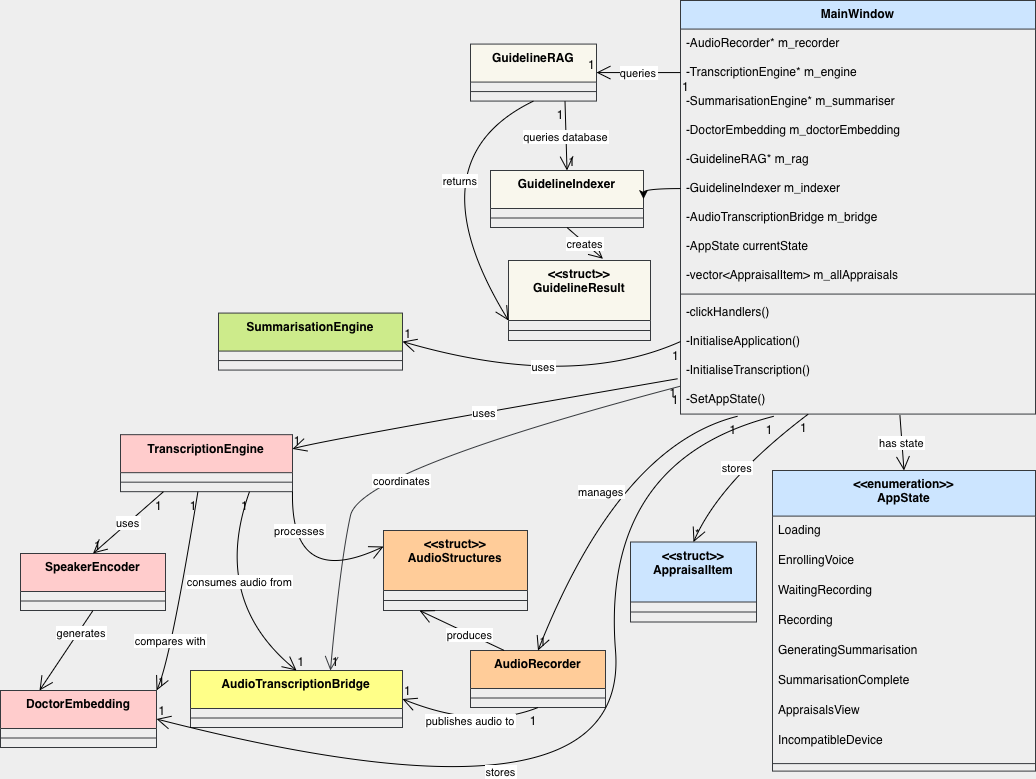
\includegraphics[width=1\linewidth]{chapters/uml_brief.drawio.png}
    \caption{This figure shows an brief overview of the classes and their interactions within the application colour coded based on the threads they occupy. All class methods and attributes except MainWindow have been removed for visual clarity}
    \label{fig:uml_brief}
\end{figure}
% TODO this has a duplicate for some reason
\section{Summarisation Engine}
\label{sec:med42testj}
\subsection{Downloading Models}
All models were downloaded and quantised using the following OpenVINO command:
\begin{verbatim}
    pip install optimum[openvino]
    optimum-cli export openvino --model <huggingface-model-name> 
                --weight-format int4 <output_directory_name>
\end{verbatim}  

\subsection{Testing Models}
To find the model that has the best trade-off between speed and accuracy, the validation set from the previous project was used to created a testing harness to evaluate each model. The \texttt{MTS-Dialog}\cite{mts-dialog} dataset contains 1,700 mock patient-doctor transcripts each with a corresponding medical summary of the conversation, with 170 samples for validation, a strong candidate for evaluating the effectiveness of each model. The dataset was created by 3 Microsoft employees to evaluate Facebook's BART-large \cite{bart} and Google's Pegasus \cite{pegasus} models fine-tuned with guided summarisation and data augmentation. 

\subsubsection{Methodology}
\label{di:test_med42}
I used the Mistral-7b, BioMistral-7b and Med42-v2-8B models for testing based on guidance from my external supervisor. Each model followed the same strategy 
\begin{enumerate}
    \item The model was quantised to int4 and was configured with \texttt{temperature=0.3} \cite{med42temp}
    \item For each validation sample, the ground truth summary, generated summary, and time taken was recorded, then saved to a CSV.
    \item BERT score was used to determine the F1, Precision, Recall metrics explained in \cite{zhang2019bertscore} to quantitatively compare the semantic accuracy of the generated summarisation against the ground truth
    \item The average time was calculated and included in the results
\end{enumerate}

This enabled a comparison between 2 key results: the inference time and accuracy. The results are as follows

\begin{figure}[H]
    \centering
    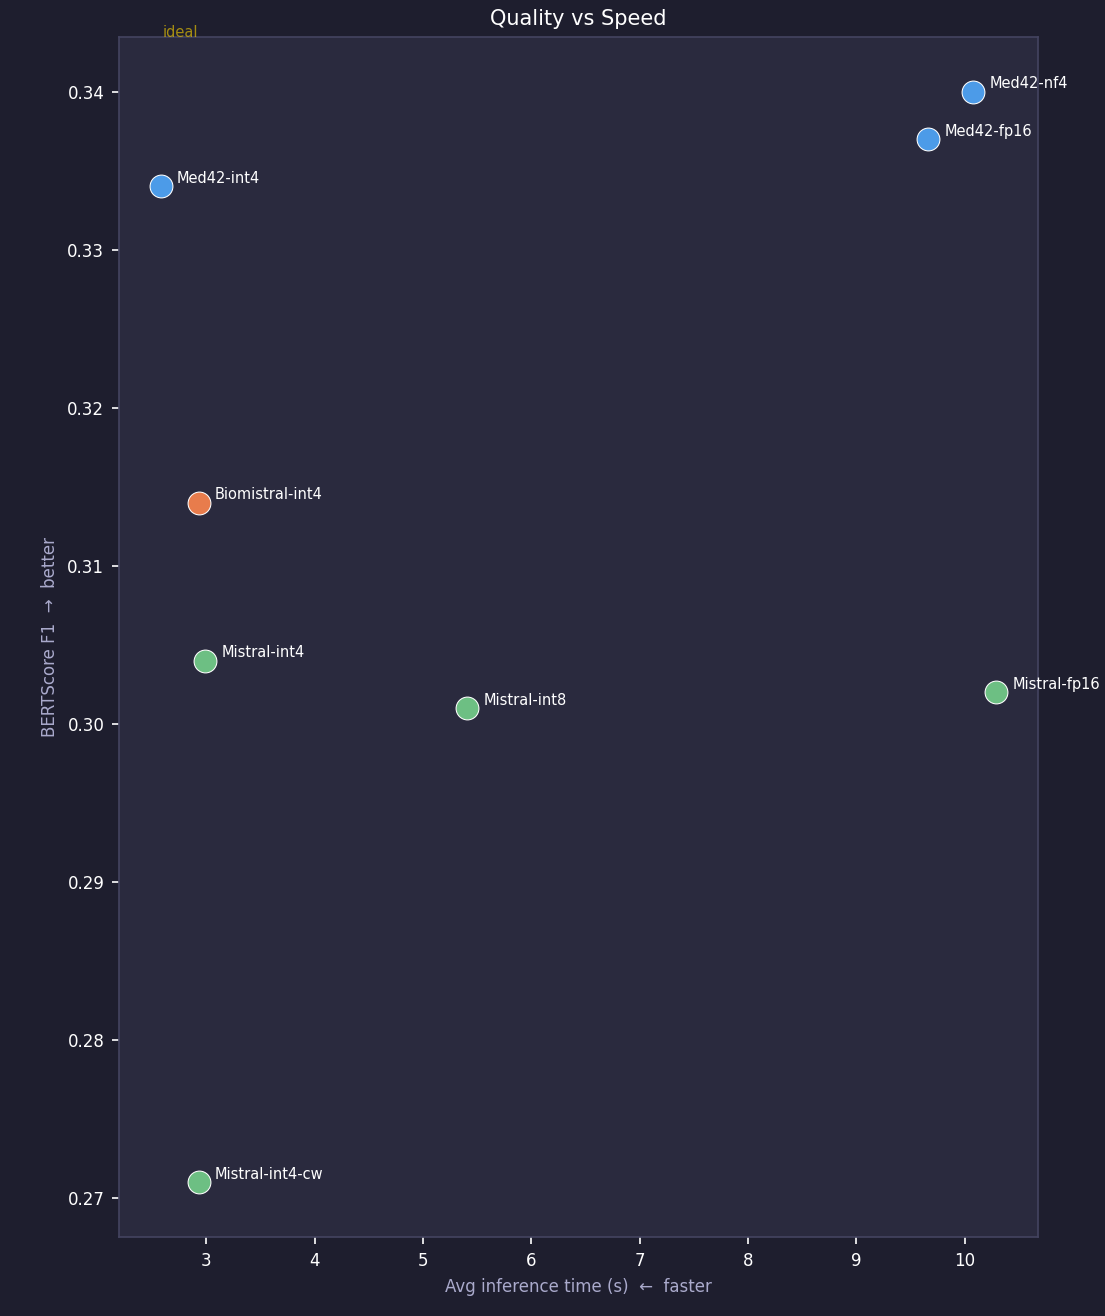
\includegraphics[width=0.75\linewidth]{model_comparison_results.png}
    \caption{A comparison between 3 models with varying quantisation levels, finding the optimal speed-accuracy tradeoff}
    \label{fig:model_comparison_results.png}
\end{figure}

We can conclude that the optimal model for this application is the Med42-v2-8B quantised to int4. As a benefit, the size of the Med42 model was reduced from 19.3GB to 4.3GB on disk.

Further testing on different devices shows the benefit of loading and running the model on the more powerful GPU compared to the NPU, resulting in the GPU being chosen for this component
\begin{figure}[htbp]
    \centering
    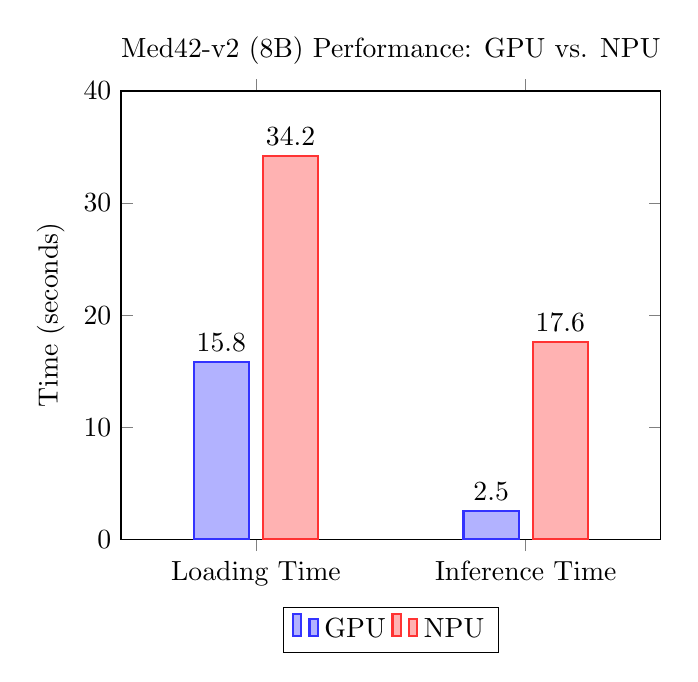
\begin{tikzpicture}
        \begin{axis}[
            ybar=5pt, % Space between the bars in a group
            bar width=20pt, % Width of the bars
            enlarge x limits=0.5, % Padding on the left and right of the chart
            legend style={at={(0.5,-0.15)}, anchor=north, legend columns=-1},
            ylabel={Time (seconds)},
            symbolic x coords={Loading Time, Inference Time}, % Swapped to be the main categories
            xtick=data,
            nodes near coords, % Displays the exact values above the bars
            nodes near coords align={vertical},
            ymin=0, ymax=40, % Normalized the height to fit the new max value (34.2)
            title={Med42-v2 (8B) Performance: GPU vs. NPU}
        ]
        
        % GPU Data (Loading, then Inference)
        \addplot[fill=blue!30, draw=blue!80, thick] coordinates {(Loading Time, 15.8) (Inference Time, 2.5)};
        
        % NPU Data (Loading, then Inference)
        \addplot[fill=red!30, draw=red!80, thick] coordinates {(Loading Time, 34.2) (Inference Time, 17.6)};
        
        \legend{GPU, NPU} % Legend now represents the hardware
        \end{axis}
    \end{tikzpicture}
    \caption{Comparison of loading and inference times for the Med42-v2 8B parameter model running on a GPU versus an NPU.}
    \label{fig:gpu_npu_performance}
\end{figure}


\subsection{Design}
\subsubsection{Concurrency}
The Med42 model requiring 20 seconds to load presents a concurrency constraint. Simply loading this model on the UI thread would cause unacceptable UI latency, therefore the following concurrency design was followed:

\begin{itemize}
    \item At program launch, a background initialisation thread is spawned to load the transcription model
    \item Once the transcription model is ready, this thread launches the Med42 summarisation model asynchronously via \texttt{std::async}, storing the result handle in a shared \texttt{std::future} member (\texttt{m\_summariserLoadFuture})
    \item An atomic boolean flag \texttt{m\_isSummariserReady} is shared between threads and set to \texttt{true} inside the async task once loading completes
    \item When the user starts recording, a separate processing thread is spawned and detached, which calls \texttt{ProcessLoop()} blocking until recording stops
    \item Once recording completes, the processing thread inspects \texttt{m\_isSummariserReady}
    \item If the model has already loaded (the common case where transcription takes longer than 20 seconds), the processing thread proceeds immediately to summary generation
    \item If the model has not yet loaded, the processing thread blocks by calling \texttt{m\_summariserLoadFuture.wait()} until the async loading task completes
    \item Once the summary is generated, the result is marshalled back to the UI thread via \texttt{DispatcherQueue().TryEnqueue()} to display
\end{itemize}

This design handles the race condition where the model has not finished loading but a transcription result arrives. Using \texttt{std::async} and \texttt{std::future} over a raw \texttt{std::thread} is preferred here because \texttt{std::future} provides a first-class blocking synchronisation primitive. The processing thread can call \texttt{wait()} directly on the future without requiring a manually managed \texttt{std::promise} or condition variable, resulting in cleaner synchronisation code.

\subsubsection{Prompting}
The effectiveness of an LLM response is highly linked to the prompt length and detail. Although pre-trained on medical textbooks and guidance, the prompt must still guide the LLM to remove any unecessary conversation and summarise only the medical facts stated to provide a history of present illness summarisation. A consultation with Dr. Tazeen Ahmed determined what was required of the summarisation resulting in the following requirements:
\begin{itemize}
    \item Facts and events must be attributed to "the doctor" or "the patient" with dates in the format DD/MM/YYYY
    \item History must be presented chronologically including onset, duration and character of pain
    \item Specific causes of injury, character of pain, aggravating factors, prior treatments and recent exacerbations must be reported
\end{itemize}

\subsection{Implementation}
The implementation is found in \texttt{SummarisationEngine.cpp}, which wraps the OpenVINO LLM pipeline with \texttt{loadModel()} and \texttt{generateFromTranscription()}

\subsubsection{Model Loading at Launch}
To launch the future from the transcription processing thread, the following implementation was chosen
\begin{verbatim}
m_summariserLoadFuture = std::async(std::launch::async, [this]() {
    try {
        m_summariser->loadModel();
        m_isSummariserReady = true;
    }
    catch (...) {
        MainWindow::SetAppState(AppState::IncompatibleDevice);
    }
});
\end{verbatim}

\texttt{std::launch::async} ensures a real OS thread is spawned. The returned \texttt{std::future<void>} is stored in the \texttt{MainWindow} member \texttt{m\_summariserLoadFuture} blocking summarisation until the task completes preventing the transcription pipeline triggering a summarisation inference before the model loads

Once loaded, the \texttt{std::atomic<bool> m\_isSummariserReady} flag is set to \texttt{true}. Should \texttt{loadModel()} throw when loading, the exception is caught and the application is moved to an \texttt{IncompatibleDevice} error state. Although the \texttt{catch} handles all error types, the only possible error when loading is a device is too little RAM or a non-Intel GPU.

\subsubsection{Waiting for the Model at Summary Time}
Once a final transcript is available, the processing thread must ensure the model is ready before calling \texttt{generateTranscription()}. It does this in two steps:

\begin{verbatim}
if (!m_isSummariserReady) {
    if (m_summariserLoadFuture.valid())
        m_summariserLoadFuture.wait();
}
\end{verbatim}

First, the atomic flag \texttt{m\_isSummariserReady} is checked. Because \texttt{std::atomic} reads are lock-free, this check is extremely cheap and covers the common case where a typical consultation lasts several minutes, well beyond the 20-second load time, so the model will almost always already be ready. If it is, execution proceeds immediately with no synchronisation overhead.

If the flag is still \texttt{false}, the thread falls through to \texttt{m\_summariserLoadFuture.wait()}. The \texttt{.valid()} guard is necessary because a default-constructed \texttt{std::future} has no associated state; calling \texttt{.wait()} on it would be undefined behaviour. \texttt{.wait()} then puts the processing thread to sleep, with no busy-waiting, until the OS wakes it once \texttt{loadModel()} returns. Critically, the UI thread is never involved in any of this waiting.

\subsubsection{Generating and Returning the Summary}
With the model guaranteed to be loaded, \texttt{generateFromTranscription()} is called synchronously on the processing thread. Once the summary string is returned, \texttt{DispatcherQueue().TryEnqueue()} marshals the result back to the UI thread for a UI update.

\subsubsection{Prompting}
The full prompt can be found in Appendix \ref{app:prompt}


